\section{Summary} \subsection{}\label{}

\begin{frame}{Learning pipeline}
	
	\begin{enumerate}
		\item Understand data and prediction goal
		\item Extract features
		\item Train Xgboost
		\item Train other models
		\item \sout{Go to sleep} Drink Café 
		\item Aggregate models
	\end{enumerate}
	
		
\end{frame}

% ---

\section{Results} \subsection{}\label{}

\begin{frame}{Results}
	
	\begin{table}[h]
		\centering
			\begin{tabular}{|c|c|}
				\hline
				Model & Score logloss \\ \hline \hline
				Mean & 0.188734 \\
				Mean by SCID & 0.143391 \\
				\hline
				One Xgboost & 0.010896 \\
				Ensemble Xgboost & 0.010724\\
				\hline
			\end{tabular}
			\label{table:cnnbenchmark}
		\end{table}
		\begin{table}[h]
			\centering
			\begin{tabular}{|c|c|}
				\hline
		1. & nbQuotesByUser\\	
		2.& max\_std\_all\_features\_byUser\\
		3. &mean\_std\_all\_features\_byUser\\
		4. &std\_broker\_AllDriversNbConvictions\\
		5. &mean\_converted\_byBroker\\
		6. &std\_broker\_countSocioDemographicId\\
		7. &nbUsersBySCID\\
		8. &std\_broker\_DeysSineCarPurchase\\
		\hline
	\end{tabular}
	\label{table:cnnbenchmark}
\end{table}
		
	
\end{frame}

\section{Some quick observations} \subsection{}\label{}

\begin{frame}{Some quick observations}
	
	\begin{figure}[H]
		\centering
		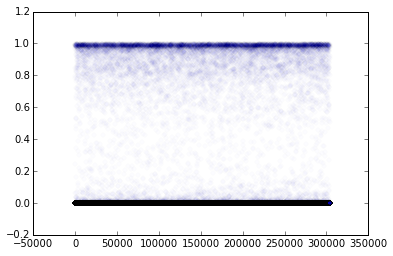
\includegraphics[width=0.7\linewidth]{images/a.png}
	\end{figure}
	
	\begin{table}[h]
		\centering
			\begin{tabular}{|c|c|c|c|c|}
				\hline
				     & >.90        & >.95       & >.99 &  Trainset \\
				     \hline
				0   & 75.59\% & 79.42\% & 92.36\% & 89.34\% \\ 
				1   & 0.24\% & 0.20\% & 7.60\% & 10.24\% \\
				2   & 0.51\% & 0.31\% & 0.05\% & 0.33\% \\
				\hline
			\end{tabular}
			\caption{abc}
			\label{table:cnnbenchmark}
		\end{table}
	
\end{frame}




